\documentclass[twoside]{book}

% Packages required by doxygen
\usepackage{fixltx2e}
\usepackage{calc}
\usepackage{doxygen}
\usepackage[export]{adjustbox} % also loads graphicx
\usepackage{graphicx}
\usepackage[utf8]{inputenc}
\usepackage{makeidx}
\usepackage{multicol}
\usepackage{multirow}
\PassOptionsToPackage{warn}{textcomp}
\usepackage{textcomp}
\usepackage[nointegrals]{wasysym}
\usepackage[table]{xcolor}

% Font selection
\usepackage[T1]{fontenc}
\usepackage[scaled=.90]{helvet}
\usepackage{courier}
\usepackage{amssymb}
\usepackage{sectsty}
\renewcommand{\familydefault}{\sfdefault}
\allsectionsfont{%
  \fontseries{bc}\selectfont%
  \color{darkgray}%
}
\renewcommand{\DoxyLabelFont}{%
  \fontseries{bc}\selectfont%
  \color{darkgray}%
}
\newcommand{\+}{\discretionary{\mbox{\scriptsize$\hookleftarrow$}}{}{}}

% Page & text layout
\usepackage{geometry}
\geometry{%
  a4paper,%
  top=2.5cm,%
  bottom=2.5cm,%
  left=2.5cm,%
  right=2.5cm%
}
\tolerance=750
\hfuzz=15pt
\hbadness=750
\setlength{\emergencystretch}{15pt}
\setlength{\parindent}{0cm}
\setlength{\parskip}{3ex plus 2ex minus 2ex}
\makeatletter
\renewcommand{\paragraph}{%
  \@startsection{paragraph}{4}{0ex}{-1.0ex}{1.0ex}{%
    \normalfont\normalsize\bfseries\SS@parafont%
  }%
}
\renewcommand{\subparagraph}{%
  \@startsection{subparagraph}{5}{0ex}{-1.0ex}{1.0ex}{%
    \normalfont\normalsize\bfseries\SS@subparafont%
  }%
}
\makeatother

% Headers & footers
\usepackage{fancyhdr}
\pagestyle{fancyplain}
\fancyhead[LE]{\fancyplain{}{\bfseries\thepage}}
\fancyhead[CE]{\fancyplain{}{}}
\fancyhead[RE]{\fancyplain{}{\bfseries\leftmark}}
\fancyhead[LO]{\fancyplain{}{\bfseries\rightmark}}
\fancyhead[CO]{\fancyplain{}{}}
\fancyhead[RO]{\fancyplain{}{\bfseries\thepage}}
\fancyfoot[LE]{\fancyplain{}{}}
\fancyfoot[CE]{\fancyplain{}{}}
\fancyfoot[RE]{\fancyplain{}{\bfseries\scriptsize Generated by Doxygen }}
\fancyfoot[LO]{\fancyplain{}{\bfseries\scriptsize Generated by Doxygen }}
\fancyfoot[CO]{\fancyplain{}{}}
\fancyfoot[RO]{\fancyplain{}{}}
\renewcommand{\footrulewidth}{0.4pt}
\renewcommand{\chaptermark}[1]{%
  \markboth{#1}{}%
}
\renewcommand{\sectionmark}[1]{%
  \markright{\thesection\ #1}%
}

% Indices & bibliography
\usepackage{natbib}
\usepackage[titles]{tocloft}
\setcounter{tocdepth}{3}
\setcounter{secnumdepth}{5}
\makeindex

% Hyperlinks (required, but should be loaded last)
\usepackage{ifpdf}
\ifpdf
  \usepackage[pdftex,pagebackref=true]{hyperref}
\else
  \usepackage[ps2pdf,pagebackref=true]{hyperref}
\fi
\hypersetup{%
  colorlinks=true,%
  linkcolor=blue,%
  citecolor=blue,%
  unicode%
}

% Custom commands
\newcommand{\clearemptydoublepage}{%
  \newpage{\pagestyle{empty}\cleardoublepage}%
}

\usepackage{caption}
\captionsetup{labelsep=space,justification=centering,font={bf},singlelinecheck=off,skip=4pt,position=top}

%===== C O N T E N T S =====

\begin{document}

% Titlepage & ToC
\hypersetup{pageanchor=false,
             bookmarksnumbered=true,
             pdfencoding=unicode
            }
\pagenumbering{alph}
\begin{titlepage}
\vspace*{7cm}
\begin{center}%
{\Large D\+NS Poisoning Tool }\\
\vspace*{1cm}
{\large Generated by Doxygen 1.8.13}\\
\end{center}
\end{titlepage}
\clearemptydoublepage
\pagenumbering{roman}
\tableofcontents
\clearemptydoublepage
\pagenumbering{arabic}
\hypersetup{pageanchor=true}

%--- Begin generated contents ---
\chapter{Namespace Index}
\section{Namespace List}
Here is a list of all documented namespaces with brief descriptions\+:\begin{DoxyCompactList}
\item\contentsline{section}{\hyperlink{namespaceDNS__Attack}{D\+N\+S\+\_\+\+Attack} \\*This package is responsible to execute all the passage required for the attack }{\pageref{namespaceDNS__Attack}}{}
\item\contentsline{section}{\hyperlink{namespaceDNS__Poisoning}{D\+N\+S\+\_\+\+Poisoning} \\*This package includes all function to execute the poisoning attack }{\pageref{namespaceDNS__Poisoning}}{}
\end{DoxyCompactList}

\chapter{Hierarchical Index}
\section{Class Hierarchy}
This inheritance list is sorted roughly, but not completely, alphabetically\+:\begin{DoxyCompactList}
\item \contentsline{section}{dns\+\_\+poisoning.\+D\+N\+S\+Poisoning}{\pageref{classdns__poisoning_1_1DNSPoisoning}}{}
\item Exception\begin{DoxyCompactList}
\item \contentsline{section}{dns\+\_\+attack.\+Initial\+Query\+Failed}{\pageref{classdns__attack_1_1InitialQueryFailed}}{}
\end{DoxyCompactList}
\end{DoxyCompactList}

\chapter{Class Index}
\section{Class List}
Here are the classes, structs, unions and interfaces with brief descriptions\+:\begin{DoxyCompactList}
\item\contentsline{section}{\hyperlink{classdns__poisoning_1_1DNSPoisoning}{dns\+\_\+poisoning.\+D\+N\+S\+Poisoning} }{\pageref{classdns__poisoning_1_1DNSPoisoning}}{}
\item\contentsline{section}{\hyperlink{classdns__attack_1_1InitialQueryFailed}{dns\+\_\+attack.\+Initial\+Query\+Failed} }{\pageref{classdns__attack_1_1InitialQueryFailed}}{}
\end{DoxyCompactList}

\chapter{Namespace Documentation}
\hypertarget{namespaceDNS__Attack}{}\section{D\+N\+S\+\_\+\+Attack Namespace Reference}
\label{namespaceDNS__Attack}\index{D\+N\+S\+\_\+\+Attack@{D\+N\+S\+\_\+\+Attack}}


This package is responsible to execute all the passage required for the attack.  




\subsection{Detailed Description}
This package is responsible to execute all the passage required for the attack. 
\hypertarget{namespaceDNS__Poisoning}{}\section{D\+N\+S\+\_\+\+Poisoning Namespace Reference}
\label{namespaceDNS__Poisoning}\index{D\+N\+S\+\_\+\+Poisoning@{D\+N\+S\+\_\+\+Poisoning}}


This package includes all function to execute the poisoning attack.  




\subsection{Detailed Description}
This package includes all function to execute the poisoning attack. 
\chapter{Class Documentation}
\hypertarget{classdns__poisoning_1_1DNSPoisoning}{}\section{dns\+\_\+poisoning.\+D\+N\+S\+Poisoning Class Reference}
\label{classdns__poisoning_1_1DNSPoisoning}\index{dns\+\_\+poisoning.\+D\+N\+S\+Poisoning@{dns\+\_\+poisoning.\+D\+N\+S\+Poisoning}}
\subsection*{Public Member Functions}
\begin{DoxyCompactItemize}
\item 
\mbox{\Hypertarget{classdns__poisoning_1_1DNSPoisoning_a2aefb588dff724bbb239fb54e2c6ca19}\label{classdns__poisoning_1_1DNSPoisoning_a2aefb588dff724bbb239fb54e2c6ca19}} 
def {\bfseries \+\_\+\+\_\+init\+\_\+\+\_\+} (self, victim\+\_\+server, spoofed\+\_\+domain, attacker\+\_\+ip, authoritative\+\_\+nameserver, initial\+\_\+id, interrupt\+\_\+handler=None, log=lambda msg\+:\+None)
\item 
\mbox{\Hypertarget{classdns__poisoning_1_1DNSPoisoning_a7208959663e75447b0221fc7fab129e7}\label{classdns__poisoning_1_1DNSPoisoning_a7208959663e75447b0221fc7fab129e7}} 
def {\bfseries send\+\_\+crafted\+\_\+packet} (self, id\+\_\+req)
\item 
\mbox{\Hypertarget{classdns__poisoning_1_1DNSPoisoning_a0c8ff9306f38db988648645b93f399d1}\label{classdns__poisoning_1_1DNSPoisoning_a0c8ff9306f38db988648645b93f399d1}} 
def {\bfseries send\+\_\+inital\+\_\+query} (self)
\item 
\mbox{\Hypertarget{classdns__poisoning_1_1DNSPoisoning_a1154be89dbdf8a2769a2ca1d3635f363}\label{classdns__poisoning_1_1DNSPoisoning_a1154be89dbdf8a2769a2ca1d3635f363}} 
def {\bfseries start\+\_\+flooding} (self)
\item 
\mbox{\Hypertarget{classdns__poisoning_1_1DNSPoisoning_aa59092cd2bd23620644af9814f782888}\label{classdns__poisoning_1_1DNSPoisoning_aa59092cd2bd23620644af9814f782888}} 
def {\bfseries check\+\_\+poisoning} (self)
\item 
\mbox{\Hypertarget{classdns__poisoning_1_1DNSPoisoning_a65f1f3e1f022f64ca35c73b80b6ccbfe}\label{classdns__poisoning_1_1DNSPoisoning_a65f1f3e1f022f64ca35c73b80b6ccbfe}} 
def {\bfseries stop\+\_\+handler} (self, sig, frame)
\end{DoxyCompactItemize}
\subsection*{Public Attributes}
\begin{DoxyCompactItemize}
\item 
\mbox{\Hypertarget{classdns__poisoning_1_1DNSPoisoning_a7ddda8f8750a3f6be247ba0aa2ae62da}\label{classdns__poisoning_1_1DNSPoisoning_a7ddda8f8750a3f6be247ba0aa2ae62da}} 
{\bfseries victim\+\_\+server}
\item 
\mbox{\Hypertarget{classdns__poisoning_1_1DNSPoisoning_a837298577cd23e34cf06ca469ab2ae77}\label{classdns__poisoning_1_1DNSPoisoning_a837298577cd23e34cf06ca469ab2ae77}} 
{\bfseries spoofed\+\_\+domain}
\item 
\mbox{\Hypertarget{classdns__poisoning_1_1DNSPoisoning_a1930111c8e62f71561f7fc808f17f306}\label{classdns__poisoning_1_1DNSPoisoning_a1930111c8e62f71561f7fc808f17f306}} 
{\bfseries attacker\+\_\+ip}
\item 
\mbox{\Hypertarget{classdns__poisoning_1_1DNSPoisoning_a96cc4f6a6168118999763b206b72cf96}\label{classdns__poisoning_1_1DNSPoisoning_a96cc4f6a6168118999763b206b72cf96}} 
{\bfseries id}
\item 
\mbox{\Hypertarget{classdns__poisoning_1_1DNSPoisoning_a5cee7b7d0614a3baade77dcf4d5db1d7}\label{classdns__poisoning_1_1DNSPoisoning_a5cee7b7d0614a3baade77dcf4d5db1d7}} 
{\bfseries sport}
\item 
\mbox{\Hypertarget{classdns__poisoning_1_1DNSPoisoning_ab54c7e8e4345d5ac1b054a2bf91aead5}\label{classdns__poisoning_1_1DNSPoisoning_ab54c7e8e4345d5ac1b054a2bf91aead5}} 
{\bfseries flood\+\_\+socket}
\item 
\mbox{\Hypertarget{classdns__poisoning_1_1DNSPoisoning_a2b7e61ab81185add0d7a97baab36924f}\label{classdns__poisoning_1_1DNSPoisoning_a2b7e61ab81185add0d7a97baab36924f}} 
{\bfseries auth\+\_\+nameserver}
\item 
\mbox{\Hypertarget{classdns__poisoning_1_1DNSPoisoning_a00a22b2725214b6052827a16b067066e}\label{classdns__poisoning_1_1DNSPoisoning_a00a22b2725214b6052827a16b067066e}} 
{\bfseries flood\+\_\+pool}
\item 
\mbox{\Hypertarget{classdns__poisoning_1_1DNSPoisoning_a9c8aa320d6ae14df500e4e04cf5f0881}\label{classdns__poisoning_1_1DNSPoisoning_a9c8aa320d6ae14df500e4e04cf5f0881}} 
{\bfseries interrupt\+\_\+handler}
\item 
\mbox{\Hypertarget{classdns__poisoning_1_1DNSPoisoning_a57e074a324e5682d4a0a0a02856c8e39}\label{classdns__poisoning_1_1DNSPoisoning_a57e074a324e5682d4a0a0a02856c8e39}} 
{\bfseries invalid\+\_\+url}
\end{DoxyCompactItemize}


The documentation for this class was generated from the following file\+:\begin{DoxyCompactItemize}
\item 
dns\+\_\+poisoning.\+py\end{DoxyCompactItemize}

\hypertarget{classdns__attack_1_1InitialQueryFailed}{}\section{dns\+\_\+attack.\+Initial\+Query\+Failed Class Reference}
\label{classdns__attack_1_1InitialQueryFailed}\index{dns\+\_\+attack.\+Initial\+Query\+Failed@{dns\+\_\+attack.\+Initial\+Query\+Failed}}


Inheritance diagram for dns\+\_\+attack.\+Initial\+Query\+Failed\+:
\nopagebreak
\begin{figure}[H]
\begin{center}
\leavevmode
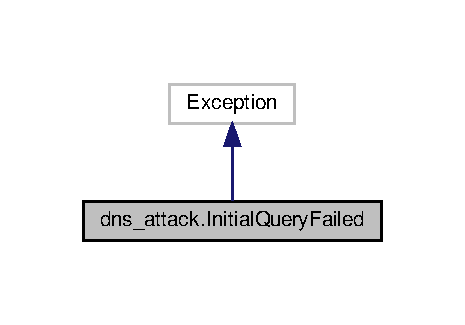
\includegraphics[width=223pt]{classdns__attack_1_1InitialQueryFailed__inherit__graph}
\end{center}
\end{figure}


Collaboration diagram for dns\+\_\+attack.\+Initial\+Query\+Failed\+:
\nopagebreak
\begin{figure}[H]
\begin{center}
\leavevmode
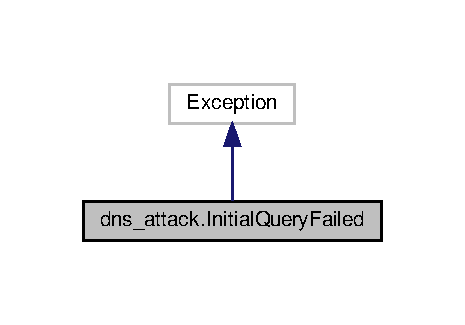
\includegraphics[width=223pt]{classdns__attack_1_1InitialQueryFailed__coll__graph}
\end{center}
\end{figure}


The documentation for this class was generated from the following file\+:\begin{DoxyCompactItemize}
\item 
dns\+\_\+attack.\+py\end{DoxyCompactItemize}

%--- End generated contents ---

% Index
\backmatter
\newpage
\phantomsection
\clearemptydoublepage
\addcontentsline{toc}{chapter}{Index}
\printindex

\end{document}
